\chapter{Besov空间}
\label{chap:besov-spaces}

第~\ref{chap:sobolev-spaces}章用可积的弱导数度量函数的光滑程度，周期阶跃函数在这把尺子上得不到任何读数：它没有一阶弱导数。可是把它平移一小步$h$，变化只发生在跳跃点附近总长约$2\lvert h\rvert$的地方，平移差的平方积分恰好等于$2\lvert h\rvert$。这条规律很整齐，而整数阶的导数条件读不出来。

还有一类信息也是导数条件读不出的。两个函数在每个尺度上的变化可能有同样的上界，其中一个在所有尺度上都顶到上界，另一个在越来越细的尺度上逐渐减弱。要区分它们，需要单独规定“各个尺度的变化怎样汇总”。本章从平移差出发，把这两类信息写成一族函数空间。

贯穿全章的图景来自第~\ref{chap:functions-as-vectors}章：把函数看成无限维向量$[\ldots,c_{j,k},\ldots]$。这里的坐标不是函数值，而是小波系数，下标$j$表示尺度，$k$表示位置，同一个$j$的坐标自然成为一组。于是Besov范数就是一种分组加权的向量范数：组内用$\ell^p$把同一尺度、不同位置的坐标合成一个数，乘上随尺度增长的权重，组间再用$\ell^q$合成最后的大小。

$s$、$p$、$q$三个参数分别管权重、组内和组间。本章前三节建立这幅图景：第~\ref{sec:besov-translation-differences}节用平移差和连续模度量变化，第~\ref{sec:besov-norms}节定义Besov范数并证明完备，第~\ref{sec:besov-wavelet}节证明差分写法与分组坐标写法等价。

有了坐标，后面的计算都成了对向量分量的操作。第~\ref{sec:besov-scale-truncation}节保留前若干组，第~\ref{sec:besov-best-n-term}节让每个函数自选最大的$N$个分量，第~\ref{sec:besov-covering}节数覆盖整个球需要多少代表。这三个问题需要的参数条件各不相同。第~\ref{sec:besov-sobolev}节回到导数，说明$B^1_{2,2}$与周期$H^1$是同一个空间。

本章只在单位周期上讨论：函数周期为$1$，积分取在一个周期$[0,1)$上，空间记为$L^p(\mathbb T)$。这样平移不受边界限制，第~\ref{chap:wavelet-transform}章的周期小波基也可以直接使用。函数默认取实值。全空间与一般区域上的Besov空间要另外处理边界和低频部分，读者可查阅函数空间理论的专著。

\section{平移差}
\label{sec:besov-translation-differences}

导数描述无穷小尺度上的变化率。若函数在某些点没有可积的导数，我们仍可以退一步，比较函数与它自身平移一小步$h$以后的差别，并观察这个差别怎样随$h$缩小。本节先用一个周期阶跃说明，平移差能读出导数条件看不到的分数次规律；再区分同一尺度上变化的大小与位置，以及不同尺度之间的汇总；最后用高阶差分和连续模把这些想法变成可以计算的量。

本章记$\Delta_hf(x)=f(x+h)-f(x)$，$f$为周期$1$的函数，$L^p$范数取在一个周期上。平移不改变$L^p(\mathbb T)$范数，这一点在后面反复使用。

\subsection{阶跃函数的平移差}
\label{sec:besov-step-differences}

取单位周期阶跃$f$：在$[0,1/2)$上为$1$，在$[1/2,1)$上为$0$，再按周期$1$延拓。它在$x=1/2$与$x=0$处跳跃，由第~\ref{chap:sobolev-spaces}章的论证，它在包含跳跃点的区间上没有弱导数，不满足一阶弱导数可积的条件。

我们直接计算平移差。设$0<h\leq1/2$。$\Delta_hf(x)\neq0$当且仅当$x$与$x+h$恰有一个落在$[0,1/2)$的周期复制中：$x\in[1/2-h,1/2)$时$f(x)=1$、$f(x+h)=0$；$x\in[1-h,1)$时$f(x)=0$、$f(x+h)=1$。在其余位置两者相同。所以$|\Delta_hf|$在总长度为$2h$的集合上等于$1$，其余为零，于是
\begin{equation}
\lVert\Delta_hf\rVert_p=(2h)^{1/p},\qquad 0<h\leq\frac12,\ 1\leq p<\infty .
\label{eq:besov-step-difference}
\end{equation}
$h<0$时把$x$换成$x+h$，得到同一结果，只需把$h$换成$|h|$。特别地，$\lVert\Delta_hf\rVert_2=(2|h|)^{1/2}$。

把它与光滑函数比较。对$g(x)=\sin(2\pi x)$，和差化积给出$\Delta_hg(x)=2\sin(\pi h)\cos(2\pi x+\pi h)$，所以$\lVert\Delta_hg\rVert_2=\sqrt2\,|\sin(\pi h)|\leq\sqrt2\,\pi|h|$。一般地，若周期函数$g$连续可微，由$\Delta_hg(x)=\int_0^hg'(x+t)\,\mathrm dt$与积分的Minkowski不等式，$\lVert\Delta_hg\rVert_p\leq|h|\,\lVert g'\rVert_p$。光滑函数的平移差与步长成正比，阶跃函数的平移差在$L^2$中只与步长的$1/2$次幂成正比。

这说明在“有可积导数”与“毫无规律”之间，还有可以检查的尺度规律：变化量是步长的分数次幂。阶跃函数虽然没有弱导数，它在$L^2$中仍有$1/2$阶的规律性。这种按步长幂次度量的规律，正是本章要刻画的光滑性。

\subsection{位置分布与尺度汇总}
\label{sec:besov-distribution-aggregation}

只给出一个幂次还不够，因为两个函数即使在小尺度上的变化有同样的上界，变化集中在哪些位置、又在多少个尺度上持续出现，仍可能不同。我们分别看这两个方面。

\paragraph{同一尺度内的位置分布}
式\eqref{eq:besov-step-difference}显示，同一个阶跃函数在不同积分指数下表现出不同的幂次：$p=1$时为$1$，$p=2$时为$1/2$，$p\to\infty$时趋于$0$。原因是变化集中在长度为$2h$的小集合上，幅度却保持为$1$。$p$越大，积分越看重少数大值，集中的变化就显得越剧烈。光滑的$\sin(2\pi x)$则不同，它的变化分散在整个周期上，对每个$p$都是$1$次。所以积分指数$p$记录了同一尺度上变化在位置上的分布。前章的积分指数已经起过类似作用，例如$W^{1,p}$是否包含某个幂函数取决于$p$；本章把这一作用与后面的尺度汇总分开规定。

\paragraph{不同尺度之间的汇总}
为看清尺度汇总，考虑单一频率的分量$u_j(x)=2^{-js}\cos(2\pi2^jx)$，$0<s<1$。与正弦函数的计算相同，
\[
\lVert\Delta_hu_j\rVert_2=2^{-js}\sqrt2\,|\sin(\pi2^jh)| .
\]
当$h$约为$2^{-j}$时，它与$2^{-js}$同阶；当$h\ll2^{-j}$时，它约为$\sqrt2\pi2^{j(1-s)}h$，小得多。所以第$j$个分量主要在尺度$h\approx2^{-j}$处“活跃”。

把这些分量按权重叠加：对$0\leq b_j\leq1$，令$f_b=\sum_{j\geq1}b_ju_j$。各分量频率不同，在$L^2$中正交，所以$\lVert\Delta_hf_b\rVert_2^2=\sum_jb_j^2\,2^{-2js}\cdot2\sin^2(\pi2^jh)$。用$|\sin\theta|\leq\min(1,|\theta|)$，把$2^jh\leq1$与$2^jh>1$的项分开求几何和，可得对每个这样的权重序列都有$\lVert\Delta_hf_b\rVert_2\leq C_sh^s$，$C_s$只依赖$s$。另一方面，取$h=2^{-J-1}$，单独第$J$项就给出$\lVert\Delta_hf_b\rVert_2\geq\sqrt2\,b_J2^{-Js}=\sqrt2\,b_J(2h)^s$。所以在尺度$2^{-J}$附近，$h^{-s}\lVert\Delta_hf_b\rVert_2$的大小主要由$b_J$及相邻几个$b_j$决定。

比较$b_j=1$与$b_j=1/j$两种权重。两个函数满足同样的统一上界$\lVert\Delta_hf_b\rVert_2\leq C_sh^s$：前者在每个二进尺度上都达到这个量级，后者在越来越细的尺度上逐渐减弱。统一上界只要求各尺度的贡献$(b_j)$有界，看不出这一区别。若进一步问这些贡献作为一个序列有多大，例如是否平方可和，两者就分开了：$(1/j)$平方可和，$(1)$不可和。所以除了同一尺度内的度量方式，还需单独规定不同尺度上的变化怎样汇总，第~\ref{sec:besov-norms}节的第二个指数承担这项工作。

\subsection{有限差分}
\label{sec:besov-finite-differences}

一阶平移差只能读出不超过一阶的规律：光滑函数的一阶差分也只与$h$成正比，读不出更高的光滑性。为读取更高阶的变化，把平移差迭代起来。对正整数$r$，定义$r$阶\term{有限差分}（finite difference）$\Delta_h^r=\Delta_h(\Delta_h^{r-1})$，$\Delta_h^1=\Delta_h$。展开得
\[
\Delta_h^rf(x)=\sum_{i=0}^r(-1)^{r-i}\binom ri f(x+ih).
\]
例如$\Delta_h^2f(x)=f(x+2h)-2f(x+h)+f(x)$。

高阶差分的作用在于抵消低阶多项式。$\Delta_h$把次数为$m$的多项式变成次数不超过$m-1$的多项式，所以$\Delta_h^r$消去所有次数小于$r$的多项式：$\Delta_hx=h$，$\Delta_h^2x=0$，$\Delta_h^2x^2=2h^2$。周期函数在整体上不是多项式，但若$f$在区间$[x,x+rh]$上与一个次数小于$r$的多项式重合，则$\Delta_h^rf(x)=0$。因此$r$阶差分忽略函数中局部的低阶多项式部分，只读出超出它的变化。

对光滑函数可以写出精确的积分表示。若周期函数$f$有$r$阶连续导数，$h>0$，对$r$归纳可得
\[
\Delta_h^rf(x)=\int_{[0,h]^r}f^{(r)}(x+t_1+\cdots+t_r)\,\mathrm dt_1\cdots\mathrm dt_r .
\]
由积分的Minkowski不等式，$\lVert\Delta_h^rf\rVert_p\leq h^r\lVert f^{(r)}\rVert_p$。另一方面，每作一次差分范数至多加倍，所以对任意$f\in L^p(\mathbb T)$都有$\lVert\Delta_h^rf\rVert_p\leq2^r\lVert f\rVert_p$。

\begin{example}[折线的二阶差分]
\label{ex:besov-triangle-wave}
令$g$为周期$1$的三角波：在$[0,1)$上$g(x)=|x-1/2|$。它连续，斜率处处为$\pm1$，在$x=1/2$和整数点有折点。一阶差分$|\Delta_hg|$在远离折点处等于$h$，所以$\lVert\Delta_hg\rVert_p$与$h$同阶，读不出比一阶更多的东西。二阶差分则只在$[x,x+2h]$包含折点时非零，这样的$x$组成总长度为$4h$的集合；在那里，由折线的凸性或凹性，$|\Delta_h^2g(x)|\leq2h$。所以$\lVert\Delta_h^2g\rVert_p\leq2h(4h)^{1/p}$，是$1+1/p$阶的。二阶差分看见了一阶差分看不见的规律：三角波除去折点处的集中变化以外，处处是线性的。
\end{example}

\subsection{连续模}
\label{sec:besov-modulus}

差分依赖一个具体的步长$h$。为了得到只依赖尺度的量，对所有不超过给定尺度的步长取最坏情形。

\begin{definition}[连续模]
\label{def:besov-modulus}
设$1\leq p\leq\infty$，$r$为正整数，$f\in L^p(\mathbb T)$。对$t>0$，称
\[
\omega_r(f,t)_p=\sup_{0<|h|\leq t}\lVert\Delta_h^rf\rVert_p
\]
为$f$在$L^p$中的$r$阶\term{连续模}（modulus of continuity）。
\end{definition}

它量化了步长不超过$t$时的统一变化。由定义，$\omega_r(f,t)_p$随$t$单调不减；由上一小节，$\omega_r(f,t)_p\leq2^r\lVert f\rVert_p$，对$r$阶连续可微的$f$还有$\omega_r(f,t)_p\leq t^r\lVert f^{(r)}\rVert_p$。差分对$f$线性，再由Minkowski不等式，$\omega_r(f+g,t)_p\leq\omega_r(f,t)_p+\omega_r(g,t)_p$。对阶跃函数，式\eqref{eq:besov-step-difference}给出$\omega_1(f,t)_p=(2t)^{1/p}$，$0<t\leq1/2$。

为什么要用高于待刻画阶数的差分？连续模的增长不能比$t^r$更慢，除非函数是常数。在$L^2$中这可以直接证明。记$\widehat f(k)=\int_0^1f(x)e^{-2\pi\mathrm ikx}\,\mathrm dx$。把第~\ref{chap:fourier-transform}章周期$2\pi$的Parseval等式换元到周期$1$，得$\lVert f\rVert_2^2=\sum_k|\widehat f(k)|^2$；平移对应于系数乘以$e^{2\pi\mathrm ikh}$，而$|e^{2\pi\mathrm ikh}-1|=2|\sin(\pi kh)|$，所以
\begin{equation}
\lVert\Delta_h^rf\rVert_2^2=\sum_{k\in\mathbb Z}\bigl(2|\sin(\pi kh)|\bigr)^{2r}|\widehat f(k)|^2 .
\label{eq:besov-difference-fourier}
\end{equation}
若$\omega_r(f,t)_2\leq\epsilon(t)t^r$且$\epsilon(t)\to0$，固定$k\neq0$，取$h=t$，只保留第$k$项，得$(2|\sin(\pi kt)|/t)^{2r}|\widehat f(k)|^2\leq\epsilon(t)^2$。令$t\to0$，左端趋于$(2\pi|k|)^{2r}|\widehat f(k)|^2$，所以$\widehat f(k)=0$。于是$f$是常数。

这个现象称为饱和：$r$阶连续模至多能表达$r$阶的规律。若想用$\omega_r(f,t)_p\leq Ct^s$刻画$s$阶光滑性，而$s>r$，那么只有常数满足条件。例如$\sin(2\pi x)$在$L^2$中有$\omega_1(\sin(2\pi\cdot),t)_2=\sqrt2\sin(\pi t)$（$t\leq1/2$），与$t$同阶，$t^{-s}\omega_1$在$s>1$时无界，尽管这个函数任意光滑。$s=r$恰好处在边界上，下一节的定义也避开它。所以刻画$s$阶光滑性时，所用差分阶数$r$必须严格大于$s$；例~\ref{ex:besov-triangle-wave}中二阶差分读出一阶差分读不出的$1+1/p$阶规律，也是这个原因。

\section{Besov范数}
\label{sec:besov-norms}

上一节得到了两类信息：连续模$\omega_r(f,t)_p$记录尺度$t$上的变化，积分指数$p$决定同一尺度内怎样度量位置不同的变化；不同尺度之间怎样汇总则尚未规定。本节把小尺度变化乘以光滑性权重$t^{-s}$，再对所有尺度统一汇总，定义Besov范数。随后用周期阶跃检验每个参数的作用，最后证明空间完备。

\subsection{差分范数}
\label{sec:besov-difference-norm}

汇总不同尺度时，要让每个尺度得到同样的分量。测度$\mathrm dt/t$满足这一点：每个二进区间$[2^{-j-1},2^{-j}]$的测度都是$\ln2$，与$j$无关。在这个测度下取$L^q$大小，就是把各尺度的贡献按$\ell^q$方式汇总。

\begin{definition}[周期Besov空间]
\label{def:besov-space}
设$1\leq p,q\leq\infty$，$s>0$，整数$r>s$。对$f\in L^p(\mathbb T)$，令
\begin{equation*}
\begin{aligned}
|f|_{B^s_{p,q}}&=\Bigl(\int_0^1\bigl(t^{-s}\omega_r(f,t)_p\bigr)^q\,\frac{\mathrm dt}{t}\Bigr)^{1/q}\quad(q<\infty),\\
|f|_{B^s_{p,\infty}}&=\sup_{0<t\leq1}t^{-s}\omega_r(f,t)_p ,
\end{aligned}
\end{equation*}
并令$\lVert f\rVert_{B^s_{p,q}}=\lVert f\rVert_p+|f|_{B^s_{p,q}}$。所有使$\lVert f\rVert_{B^s_{p,q}}<\infty$的$f\in L^p(\mathbb T)$组成的空间称为周期\term{Besov空间}（Besov space），记为$B^s_{p,q}(\mathbb T)$，简记为$B^s_{p,q}$。
\end{definition}

定义中$t^{-s}\omega_r(f,t)_p$是尺度$t$上的变化相对于期望量级$t^s$的比值，$|f|_{B^s_{p,q}}$把这些比值按$\ell^q$方式汇总。只取$t\leq1$是因为周期为$1$，更大的步长不提供新信息；大尺度的大小由$\lVert f\rVert_p$记录。不同的$r>s$给出等价的范数，所以空间不依赖$r$的选择，这一点这里不给出证明。

由于$\omega_r$单调，积分形式可以换成离散的二进和。对$t\in[2^{-j-1},2^{-j}]$，$\omega_r(f,2^{-j-1})_p\leq\omega_r(f,t)_p\leq\omega_r(f,2^{-j})_p$，且$2^{js}\leq t^{-s}\leq2^{(j+1)s}$，每段的$\mathrm dt/t$测度为$\ln2$。逐段估计后求和，得
\begin{equation}
2^{-sq}\ln2\sum_{j\geq1}\bigl(2^{js}\omega_r(f,2^{-j})_p\bigr)^q\leq|f|_{B^s_{p,q}}^q\leq2^{sq}\ln2\sum_{j\geq0}\bigl(2^{js}\omega_r(f,2^{-j})_p\bigr)^q ,
\label{eq:besov-dyadic-form}
\end{equation}
$q=\infty$时把和换成上确界。$j=0$的项不超过$2^r\lVert f\rVert_p$，已被范数的$L^p$部分控制。所以$|f|_{B^s_{p,q}}$与序列$(2^{js}\omega_r(f,2^{-j})_p)_{j\geq0}$的$\ell^q$范数相差有界倍数。

离散形式立即给出两类包含关系。若$q_1\leq q_2$，由$\ell^{q_1}\subset\ell^{q_2}$，$B^s_{p,q_1}\subset B^s_{p,q_2}$：汇总指数越小，要求越严。若$s'<s$，对任意$q$，$(2^{js'}\omega_r)^q=2^{-j(s-s')q}(2^{js}\omega_r)^q$，后一因子有界时前者可和，所以$B^s_{p,\infty}\subset B^{s'}_{p,q}$：降低一点光滑阶数，就可以换取任意的汇总方式。改变$q$只改变允许的尺度分布，改变$s$则改变每个尺度上期望的量级。

\subsection{参数的作用}
\label{sec:besov-parameters}

三个参数分工明确：$s$规定期望的变化阶数，$p$汇总同一尺度内不同位置的变化，$q$汇总不同尺度的变化。我们用周期阶跃$f$检验这一分工。固定$p=2$与$0<s<1$，此时可以取$r=1$。

由式\eqref{eq:besov-step-difference}，$0<t\leq1/2$时$\omega_1(f,t)_2=(2t)^{1/2}$。$1/2<t\leq1$时，取$h=1/2$得到$\lVert\Delta_hf\rVert_2=1$；而$1/2<h\leq1$时，周期性给出$\Delta_hf=\Delta_{h-1}f$，其范数$(2(1-h))^{1/2}\leq1$，所以$\omega_1(f,t)_2=1$。代入定义，$[1/2,1]$上的部分总是有限，关键是$t\to0$的部分：
\[
\int_0^{1/2}\bigl(t^{-s}(2t)^{1/2}\bigr)^q\,\frac{\mathrm dt}{t}=2^{q/2}\int_0^{1/2}t^{q(1/2-s)-1}\,\mathrm dt .
\]

当$s<1/2$时，指数$q(1/2-s)-1>-1$，积分对每个有限$q$都有限，$q=\infty$时上确界也有限。所以阶跃函数属于每个$B^s_{2,q}$，$0<s<1/2$。当$s=1/2$时，被积函数为$2^{q/2}t^{-1}$，积分对每个有限$q$都发散；而$q=\infty$时，$\sup_tt^{-1/2}\omega_1(f,t)_2=\sqrt2$有限。所以阶跃函数属于$B^{1/2}_{2,\infty}$，不属于任何$q<\infty$的$B^{1/2}_{2,q}$。当$s>1/2$时，$t^{-s}(2t)^{1/2}\to\infty$，阶跃函数不属于任何$B^s_{2,q}$。

这三种情形看清了$s$与$q$各自的作用。$s$决定比较的基准$t^s$：$s<1/2$时阶跃函数在每个尺度上的变化都比基准小得多，并且越细越小，任何汇总方式都可以接受；$s>1/2$时变化比基准大，无论怎样汇总都不行。$s=1/2$恰好是阶跃函数的变化阶数，此时每个二进尺度贡献大小相同的比值$\sqrt2$，只有不要求跨尺度可和的$q=\infty$能够接受。上一节的$f_b$也是如此：在$B^s_{2,q}$中的成员资格大致取决于权重序列$(b_j)$是否属于$\ell^q$。

积分指数$p$的作用也可以从同一个函数读出。由式\eqref{eq:besov-step-difference}，$\omega_1(f,t)_p=(2t)^{1/p}$，所以同样的论证说明阶跃函数属于$B^{1/p}_{p,\infty}$，并属于每个$s<1/p$的$B^s_{p,q}$。$p=1$时阶数为$1$，$p$越大阶数越低：变化集中在小集合上，积分指数越高，这种集中就被看得越重。对比之下，阶跃函数不属于任何$W^{1,p}$；Besov尺度给了它一个确切的位置。

\subsection{完备性}
\label{sec:besov-completeness}

先核对$\lVert\cdot\rVert_{B^s_{p,q}}$是范数。齐次性显然。差分对函数线性，由上一节$\omega_r(f+g,t)_p\leq\omega_r(f,t)_p+\omega_r(g,t)_p$，再对$L^q(\mathrm dt/t)$用Minkowski不等式（$q=\infty$时直接取上确界），得$|f+g|_{B^s_{p,q}}\leq|f|_{B^s_{p,q}}+|g|_{B^s_{p,q}}$。所以Besov条件对加法和数乘封闭，$B^s_{p,q}$是线性空间。若$\lVert f\rVert_{B^s_{p,q}}=0$，则$\lVert f\rVert_p=0$，$f$是零等价类；单独的$|\cdot|_{B^s_{p,q}}$只是半范数，在常数上为零，$L^p$项正是为排除这一点而加入的。

\begin{theorem}[Besov空间的完备性]
\label{thm:besov-complete}
设$1\leq p,q\leq\infty$，$s>0$，整数$r>s$。则$B^s_{p,q}(\mathbb T)$是Banach空间。
\end{theorem}

\begin{proof}
设$(f_n)$是$B^s_{p,q}$中的Cauchy列。由$\lVert f_n-f_m\rVert_p\leq\lVert f_n-f_m\rVert_{B^s_{p,q}}$，它也是$L^p$中的Cauchy列，由$L^p$的完备性收敛到某个$f\in L^p(\mathbb T)$。

下面控制$f-f_m$的差分。固定$m$与$h$。由$\lVert\Delta_h^rg\rVert_p\leq2^r\lVert g\rVert_p$，差分在$L^p$中连续，所以$\Delta_h^r(f_n-f_m)\to\Delta_h^r(f-f_m)$，从而
\begin{equation*}
\begin{aligned}
\lVert\Delta_h^r(f-f_m)\rVert_p&=\lim_{n\to\infty}\lVert\Delta_h^r(f_n-f_m)\rVert_p\\
&\leq\liminf_{n\to\infty}\omega_r(f_n-f_m,t)_p,\qquad|h|\leq t .
\end{aligned}
\end{equation*}
对$|h|\leq t$取上确界，得$\omega_r(f-f_m,t)_p\leq\liminf_n\omega_r(f_n-f_m,t)_p$。乘以$t^{-s}$后，$q<\infty$时由Fatou引理，$q=\infty$时直接取上确界，得
\[
|f-f_m|_{B^s_{p,q}}\leq\liminf_{n\to\infty}|f_n-f_m|_{B^s_{p,q}} .
\]

任给$\varepsilon>0$，取$M$使$m,n\geq M$时$\lVert f_n-f_m\rVert_{B^s_{p,q}}<\varepsilon$。则$m\geq M$时$|f-f_m|_{B^s_{p,q}}\leq\varepsilon$，并且$\lVert f-f_m\rVert_p=\lim_n\lVert f_n-f_m\rVert_p\leq\varepsilon$。于是$f=f_m+(f-f_m)\in B^s_{p,q}$，且$\lVert f-f_m\rVert_{B^s_{p,q}}\leq2\varepsilon$，即$f_m\to f$在$B^s_{p,q}$中成立。
\end{proof}

证明的结构与Sobolev空间的完备性相似：先在较弱的$L^p$中取得极限，再说明附加的条件在极限中保留。不同之处在于，这里附加的条件不是测试恒等式，而是对每个步长的差分估计，它通过差分在$L^p$中的连续性与Fatou引理传到极限。

\section{小波刻画}
\label{sec:besov-wavelet}

差分范数直接表达了“尺度$t$上的变化”，但用它计算逼近误差并不方便：误差要求知道函数由哪些成分组成，连续模只给出整体的变化量。小波基给出函数的坐标，第$j$层系数正好对应尺度$2^{-j}$附近、不同位置上的变化。本节把差分范数改写成对坐标的条件，后面三节都在这组坐标中计算。

\paragraph{周期小波基与系数}
由第~\ref{chap:wavelet-transform}章，取实值的紧支撑正交多分辨率分析，尺度函数$\varphi$与母小波$\psi$都支撑在$[0,L]$中，令$\varphi_{j,k}(x)=2^{j/2}\varphi(2^jx-k)$，$\psi_{j,k}$同理，再沿整数平移求和得到周期基函数。为简洁，本章省去周期化的上标。

固定起始尺度$j_0\geq0$，并要求$2^{j_0}\geq L$，使每个$\psi_{j,k}$（$j\geq j_0$）的支撑在一个周期内不与自身的平移重叠。由第~\ref{chap:wavelet-transform}章的周期小波基定理，下面的函数族是$L^2(\mathbb T)$的标准正交基：
\[
 \{\varphi_{j_0,k}:0\leq k<2^{j_0}\}\cup\{\psi_{j,k}:j\geq j_0,\ 0\leq k<2^j\}.
\]

基函数有界，所以对$f\in L^p(\mathbb T)\subset L^1(\mathbb T)$可以用积分读取系数。粗项系数记为$a_k$，第$j$层细节系数记为$c_{j,k}$：
\[
 a_k=\int_0^1f\varphi_{j_0,k},\qquad c_{j,k}=\int_0^1f\psi_{j,k} .
\]
记$a=(a_k)_{0\leq k<2^{j_0}}$，$c_j=(c_{j,k})_{0\leq k<2^j}$。对$f\in L^2(\mathbb T)$，Parseval等式给出
\[
 \lVert f\rVert_2^2=\lVert a\rVert_{\ell^2}^2+\sum_{j\geq j_0}\lVert c_j\rVert_{\ell^2}^2 .
\]

这样每个函数就对应一个分组的无限维向量$[a\mid c_{j_0}\mid c_{j_0+1}\mid\cdots]$，第$j$组有$2^j$个分量。

\paragraph{贯穿后文的例子}
后面三节用一个能手算的函数：$f=\mathbf 1_{[0,1/3)}$按周期$1$延拓，用Haar基，$j_0=0$，$a_0=\int_0^1f=1/3$。跳跃点$1/3$不在任何二进分点上，这正是选它的原因；若跳在$1/2$，Haar展开只有一项，不具代表性。周期平移差与上一节相同，当$\lvert h\rvert\leq1/3$时$\lVert\Delta_hf\rVert_2=(2\lvert h\rvert)^{1/2}$。

计算第$j$层的系数。若$\psi_{j,k}$的支撑不含$1/3$，则$f$在支撑上是常数，由$\int\psi_{j,k}=0$可知系数为零。所以每层只有一个非零系数，位于$k_j=\lfloor2^j/3\rfloor$。令$\theta=2^j/3-k_j$，则$j$为偶数时$\theta=1/3$，$j$为奇数时$\theta=2/3$。

在这个区间上，$f$只在相对位置$[0,\theta)$上等于$1$。$\psi_{j,k_j}$在左半取值$2^{j/2}$、右半取值$-2^{j/2}$，区间长度为$2^{-j}$，所以
\[
 c_{j,k_j}=2^{-j/2}\Bigl(\int_0^\theta\mathbf 1_{[0,1/2)}-\int_0^\theta\mathbf 1_{[1/2,1)}\Bigr)=\frac{2^{-j/2}}{3},
\]
$\theta=1/3$时括号内是$1/3$，$\theta=2/3$时括号内是$1/2-1/6=1/3$。

用Parseval等式核对：坐标的平方和为
\[
 \frac19+\sum_{j\geq0}\frac{2^{-j}}{9}=\frac19+\frac29=\frac13=\lVert f\rVert_2^2 .
\]

\subsection{单尺度系数的大小}
\label{sec:besov-single-scale}

先看一组坐标怎样对应函数的大小。$\psi_{j,k}$在$L^2$中归一化，其$L^p$范数却随尺度变化。换元$y=2^jx-k$给出
\begin{equation}
 \lVert\psi_{j,k}\rVert_p=2^{j/2}\Bigl(\int\lvert\psi(2^jx-k)\rvert^p\,\mathrm dx\Bigr)^{1/p}=2^{j(1/2-1/p)}\lVert\psi\rVert_p .
 \label{eq:besov-psi-lp}
\end{equation}
$p=2$时因子为$1$；$p<2$时细尺度上单个小波的$L^p$范数变小，$p>2$时变大。这是$L^2$归一化与$L^p$度量之间的换算，与函数的光滑性无关。

同一层的小波支撑长度为$L2^{-j}$，每点至多被有限个支撑覆盖，所以一层的组合大致是这些“块”的不交拼接，其$L^p$范数应当与单块范数乘以系数的$\ell^p$范数相当。这正是分组向量的“组内$\ell^p$”的来源。

\begin{lemma}[单层组合的$L^p$大小]
\label{lem:besov-single-level}
设$1\leq p\leq\infty$，$j\geq j_0$。存在只依赖$\psi$、$L$与$p$的常数$0<c\leq C$，使对任意系数$(c_k)_{0\leq k<2^j}$，函数$g=\sum_kc_k\psi_{j,k}$满足
\begin{equation}
 c\,2^{j(1/2-1/p)}\lVert(c_k)\rVert_{\ell^p}\leq\lVert g\rVert_p\leq C\,2^{j(1/2-1/p)}\lVert(c_k)\rVert_{\ell^p} .
 \label{eq:besov-single-level}
\end{equation}
\end{lemma}

\begin{proof}
记$m=\lceil L\rceil+1$，每点至多属于$m$个支撑$I_k=\operatorname{supp}\psi_{j,k}$。先设$p<\infty$。

上界：在每点只有至多$m$个非零项，由有限和的Hölder不等式，
\[
 \lvert g(x)\rvert^p\leq m^{p-1}\sum_k\lvert c_k\rvert^p\lvert\psi_{j,k}(x)\rvert^p .
\]
积分后用式~\eqref{eq:besov-psi-lp}，得到
\[
 \lVert g\rVert_p^p\leq m^{p-1}\lVert\psi\rVert_p^p\,2^{j(p/2-1)}\sum_k\lvert c_k\rvert^p .
\]

下界：由正交性，$c_k=\int_{I_k}g\psi_{j,k}$。记$p'$为$p$的共轭指数，Hölder不等式给出
\[
 \lvert c_k\rvert\leq\lVert g\rVert_{L^p(I_k)}\lVert\psi_{j,k}\rVert_{p'}=\lVert g\rVert_{L^p(I_k)}\,2^{j(1/p-1/2)}\lVert\psi\rVert_{p'}.
\]

取$p$次方后对$k$求和，每点至多被计入$m$次，于是
\[
 \sum_k\lvert c_k\rvert^p\leq m\,2^{j(1-p/2)}\lVert\psi\rVert_{p'}^p\lVert g\rVert_p^p.
\]
两边开$p$次方，就是所要的下界。$p=\infty$时把求和换成最大值，论证相同。
\end{proof}

上界只用到支撑的重叠次数和$\psi$有界，把$\psi$换成其他紧支撑有界函数仍然成立，下一小节要用这一点。

\paragraph{手算：集中与分散}
对Haar小波，同层支撑两两不交，$\lvert\psi_{j,k}\rvert$在支撑上恒为$2^{j/2}$，式~\eqref{eq:besov-single-level}两端恰好相等。取$j=3$，比较两组$\ell^2$范数都是$1$的系数：
\[
 c^{\mathrm A}=(1,0,\ldots,0),\qquad c^{\mathrm B}=\frac{1}{\sqrt8}(1,\ldots,1).
\]

$c^{\mathrm A}$的能量集中在一个位置，对应的函数是高为$2^{3/2}$的窄脉冲。$c^{\mathrm B}$的能量分散到全部$8$个位置，对应的函数在每点取值$\pm1$。把它们的组内范数代入式~\eqref{eq:besov-single-level}，结果列在表~\ref{tab:besov-concentrate-spread}中。

\begin{BookInlineTable}
  \centering
  \begin{tabular}{@{}llll@{}}
    \toprule
    & $p=1$ & $p=2$ & $p=\infty$\\
    \midrule
    因子$2^{3(1/2-1/p)}$ & $2^{-3/2}$ & $1$ & $2^{3/2}$\\
    $\lVert c^{\mathrm A}\rVert_{\ell^p}$ & $1$ & $1$ & $1$\\
    $\lVert c^{\mathrm B}\rVert_{\ell^p}$ & $2^{3/2}$ & $1$ & $2^{-3/2}$\\
    $\lVert g^{\mathrm A}\rVert_p$ & $0.354$ & $1$ & $2.83$\\
    $\lVert g^{\mathrm B}\rVert_p$ & $1$ & $1$ & $1$\\
    \bottomrule
  \end{tabular}
  \caption{同一层上两组系数的$L^p$大小。集中的系数在$p$较大时显得大，分散的系数对各个$p$相同。}
  \label{tab:besov-concentrate-spread}
\end{BookInlineTable}

\begin{BookInlineFigure}
  \centering
  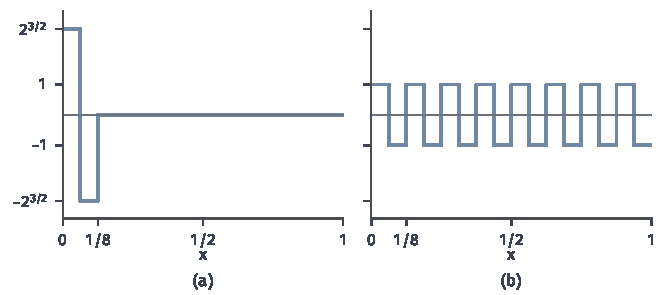
\includegraphics[width=112mm]{figures/04-spaces-measures-and-geometry/03-function-spaces/matplotlib/besov-lp-position/figure.pdf}
  \caption{第$3$层Haar组合。(a)系数集中：$g^{\mathrm A}=\psi_{3,0}$，是一个高$2^{3/2}$、宽$1/8$的脉冲。(b)系数分散：$g^{\mathrm B}=8^{-1/2}\sum_k\psi_{3,k}$，处处$\lvert g^{\mathrm B}\rvert=1$。两者系数的$\ell^2$范数相同。}
  \label{fig:besov-lp-position}
\end{BookInlineFigure}

图~\ref{fig:besov-lp-position}解释了这张表。$L^2$看不出区别，$L^\infty$只看峰值，脉冲因此显得大，$L^1$看总面积，脉冲因此显得小。$2^{j(1/2-1/p)}\lVert c_j\rVert_{\ell^p}$正是第$j$层细节在$L^p$中的大小，$\ell^p$范数把差分范数中“同一尺度、不同位置”的汇总搬到了坐标上。

再乘以$2^{js}$，就把这一层的大小与期望量级$2^{-js}$相比较，对应差分范数中的$t^{-s}$。粗项$a$只有$2^{j_0}$个分量，记录最大尺度上的整体大小，对应差分范数中的$\lVert f\rVert_p$；它不能省略，否则常数函数会得到零范数。

\subsection{小波等价范数}
\label{sec:besov-wavelet-norm}

把上述加权块大小按$\ell^q$汇总，就得到候选的系数范数。记
\begin{equation}
 b_j=2^{j(s+1/2-1/p)}\lVert c_j\rVert_{\ell^p},\qquad j\geq j_0 ,
 \label{eq:besov-block}
\end{equation}
并令
\begin{equation}
 \lVert f\rVert_{B^s_{p,q}}^{\mathrm w}=\lVert a\rVert_{\ell^p}+\bigl\lVert(b_j)_{j\geq j_0}\bigr\rVert_{\ell^q},
 \label{eq:besov-wavelet-norm}
\end{equation}
其中$q=\infty$时取上确界。

图~\ref{fig:besov-group-coordinates}是这个范数的计算过程。它与有限维的分组范数只有两点不同：组数无穷，组的长度$2^j$随下标增长。权重中的$s$体现光滑性要求，$1/2-1/p$只是归一化换算。

\begin{BookInlineFigure}
  \centering
  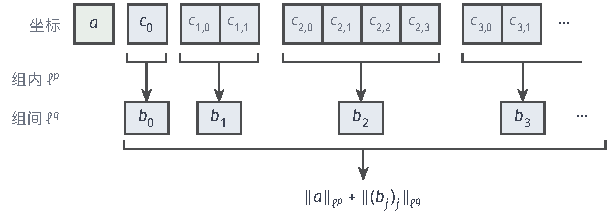
\includegraphics[width=103.3mm]{figures/04-spaces-measures-and-geometry/03-function-spaces/tikz/besov-group-coordinates/figure.pdf}
  \caption{Besov范数是分组加权的向量范数（图中取$j_0=0$）。第一行是函数的小波坐标，蓝色方格按尺度分组，第$j$组有$2^j$个分量，绿色方格是粗项。第二行把每组用$\ell^p$范数合成一个数，并乘以权重，得到式~\eqref{eq:besov-block}的$b_j$。最后对各组的$b_j$取$\ell^q$范数，再加上粗项。}
  \label{fig:besov-group-coordinates}
\end{BookInlineFigure}

用贯穿的例子算一次。取$p=2$、$q=2$、$s=1/4$，此时权重为$2^{j/4}$，每组只有一个非零坐标，所以
\[
 b_j=2^{j/4}\cdot\frac{2^{-j/2}}{3}=\frac{2^{-j/4}}{3}.
\]
前几项约为$0.333$、$0.280$、$0.236$、$0.198$。

对$b_j^2$求几何和，再加上粗项，得到
\[
 \lVert(b_j)\rVert_{\ell^2}^2=\frac{1/9}{1-2^{-1/2}}\approx0.3794,\qquad\lVert f\rVert^{\mathrm w}_{B^{1/4}_{2,2}}=\frac13+\sqrt{0.3794}\approx0.949 .
\]
若取$s=1/2$，则$b_j=1/3$对所有$j$成立，序列有界而不可和，与差分计算得到的式~\eqref{eq:besov-step-membership}一致。

\begin{theorem}[小波刻画]
\label{thm:besov-wavelet-characterization}
设$1\leq p,q\leq\infty$，$s>0$。设$\varphi$与$\psi$有直到$m$阶的连续导数且$m>s$，$\psi$有$M>s$个消失矩，即$\int x^i\psi(x)\,\mathrm dx=0$对$0\leq i<M$成立，$m$与$M$为整数。则存在常数$C_0\geq1$，使对每个$f\in L^p(\mathbb T)$，
\begin{equation}
 C_0^{-1}\lVert f\rVert_{B^s_{p,q}}^{\mathrm w}\leq\lVert f\rVert_{B^s_{p,q}}\leq C_0\lVert f\rVert_{B^s_{p,q}}^{\mathrm w},
 \label{eq:besov-wavelet-equivalence}
\end{equation}
两端同时有限或同时无限。$C_0$依赖$s,p,q$、所选小波与$j_0$。
\end{theorem}

下面写出证明的主要步骤，并分开说明两个方向分别依赖小波的哪种性质。证明中有三处引用外部事实：差分范数不依赖$r$，一般$r$的局部多项式逼近估计，以及$p<2$时小波展开在$L^p$中的收敛。取$r=\lfloor s\rfloor+1$，由$m,M$是大于$s$的整数，得到$s<r\leq\min(m,M)$。记
\[
 g_j=\sum_kc_{j,k}\psi_{j,k},\quad B_j=2^{j(1/2-1/p)}\lVert c_j\rVert_{\ell^p},\quad b_j=2^{js}B_j .
\]

\paragraph{由系数控制差分：正则性}
设系数范数有限。由引理~\ref{lem:besov-single-level}，$\lVert g_j\rVert_p\leq CB_j=C2^{-js}b_j$，而$(b_j)$有界，所以$\sum_jg_j$在$L^p$中绝对收敛，它的系数就是$f$的系数。系数全为零的$L^p$函数只有零：$p\geq2$时这是$L^2$基的完备性，$p<2$时需要用尺度函数核的估计说明投影$P_J$在$L^p$上一致有界。于是$f$等于这个级数。

对单层作差分。小步长用导数，大步长用$2^r$。$g_j^{(r)}$是由$2^{jr}(\psi^{(r)})_{j,k}$组合成的，由引理证明的上界部分，有$\lVert g_j^{(r)}\rVert_p\leq C2^{jr}B_j$。代入式~\eqref{eq:besov-difference-bounds}，得到
\[
 \lVert\Delta_h^rg_j\rVert_p\leq C\min\bigl(1,(2^j\lvert h\rvert)^r\bigr)B_j .
\]

粗项同理，只是因子$2^{jr}$换成常数。对$\lvert h\rvert\leq2^{-J}$求和，把$j<J$与$j\geq J$分开：
\[
 \omega_r(f,2^{-J})_p\leq C\Bigl(2^{-Jr}\lVert a\rVert_{\ell^p}+\sum_{j<J}2^{(j-J)r}B_j+\sum_{j\geq J}B_j\Bigr).
\]

两边乘以$2^{Js}$。用$B_j=2^{-js}b_j$改写，得到
\[
 \begin{aligned}
 2^{Js}\omega_r(f,2^{-J})_p\leq C\Bigl(&2^{-J(r-s)}\lVert a\rVert_{\ell^p}\\
 &+\sum_{j<J}2^{-(J-j)(r-s)}b_j+\sum_{j\geq J}2^{-(j-J)s}b_j\Bigr).
 \end{aligned}
\]

右端是序列$(b_j)$与一个几何衰减序列的卷积。对卷积用$\ell^q$的Minkowski不等式：若$e_J\leq\sum_n\kappa_nb_{J+n}$，$\kappa_n\geq0$，则
\begin{equation}
 \lVert(e_J)\rVert_{\ell^q}\leq\Bigl(\sum_n\kappa_n\Bigr)\lVert(b_j)\rVert_{\ell^q}.
 \label{eq:besov-convolution}
\end{equation}

这里两侧的几何比是$2^{-(r-s)}$和$2^{-s}$，两者都小于$1$，恰好需要$0<s<r$。所以序列$(2^{Js}\omega_r(f,2^{-J})_p)_{J\geq j_0}$的$\ell^q$范数不超过$C(\lVert a\rVert_{\ell^p}+\lVert(b_j)\rVert_{\ell^q})$。$J<j_0$只有有限项，每项不超过$2^r\lVert f\rVert_p$。再代入式~\eqref{eq:besov-dyadic-form}，就得到式~\eqref{eq:besov-wavelet-equivalence}的右半部分。

\paragraph{由差分控制系数：消失矩}
设$\lVert f\rVert_{B^s_{p,q}}<\infty$。先写出通用的一步。把$f$看成实轴上的周期函数，由第~\ref{chap:wavelet-transform}章的展开公式，$c_{j,k}=\int_{\mathbb R}f\psi_{j,k}$，积分区域是实轴上的支撑$I_k$，长度$\delta=L2^{-j}$。因此消失矩可以在实轴上使用，无需担心跨周期接缝。

对次数小于$r\leq M$的多项式$P_k$，有$\int P_k\psi_{j,k}=0$。于是
\[
 c_{j,k}=\int_{I_k}(f-P_k)\psi_{j,k} .
\]
用Hölder不等式与式~\eqref{eq:besov-psi-lp}，再按$k$求和，得到
\[
 B_j^p\leq\lVert\psi\rVert_{p'}^p\sum_k\lVert f-P_k\rVert_{L^p(I_k)}^p .
\]

现在要选$P_k$使右端小。$r=1$时，即$0<s<1$，$P_k$取$f$在$I_k$上的平均值。由Jensen不等式，
\[
 \lvert f(x)-P_k\rvert^p\leq\frac1\delta\int_{I_k}\lvert f(x)-f(y)\rvert^p\,\mathrm dy .
\]

对$x\in I_k$积分并换元$y=x+h$，得到
\[
 \lVert f-P_k\rVert_{L^p(I_k)}^p\leq\frac1\delta\int_{\lvert h\rvert\leq\delta}\int_{I_k}\lvert\Delta_hf(x)\rvert^p\,\mathrm dx\,\mathrm dh .
\]
对$k$求和，每点至多被计入$m$次，$\mathrm dh$的积分域长度为$2\delta$，于是
\[
 \sum_k\lVert f-P_k\rVert_{L^p(I_k)}^p\leq2m\,\omega_1(f,\delta)_p^p .
\]

由$\Delta_{nh}u=\sum_{i<n}\Delta_hu(\cdot+ih)$，得到$\omega_1(f,nt)_p\leq n\,\omega_1(f,t)_p$，所以$B_j\leq C\omega_1(f,2^{-j})_p$。乘以$2^{js}$，取$\ell^q$，由式~\eqref{eq:besov-dyadic-form}，第二项受$\lVert f\rVert_{B^s_{p,q}}$控制。粗项由同样的Hölder估计得到$\lVert a\rVert_{\ell^p}\leq C\lVert f\rVert_p$。这就完成了$0<s<1$时的左半部分。$p=\infty$时把积分换成上确界，论证相同。

$r\geq2$时机制相同，平均值换成局部的最佳多项式逼近，所需的不等式是Whitney估计，它用$r$阶差分在$I_k$附近的平均控制局部多项式逼近误差，证明较长，读者可查阅逼近论的专著。没有足够的消失矩，光滑函数在细尺度上的系数就不会足够小。

\paragraph{条件不能省略}
Haar小波给出具体的反例。Haar母小波是阶跃型函数，由式~\eqref{eq:besov-step-membership}（平移与伸缩只改变常数），它在$p=2$、$s>1/2$时不属于任何$B^s_{2,q}$，在$s=1/2$时只属于$B^{1/2}_{2,\infty}$。可是在式~\eqref{eq:besov-wavelet-norm}中，单个Haar小波只有一个非零系数，系数范数有限。所以对这些参数，Haar系数范数与差分范数不可能等价。

Haar小波在$p=2$、$0<s<1/2$时仍然适用。消失矩的方向只用$r=1$，上面的证明不变。正则性的方向要改一步：第$j$层的Haar组合是网格宽度$2^{-j-1}$上的阶梯函数，$\lVert\Delta_hg_j\rVert_2$只有$(2^j\lvert h\rvert)^{1/2}$的增益，卷积的几何比变成$2^{-(1/2-s)}$，这要求$s<1/2$。这也是本章手算例子可以用Haar基的依据，手算的结果只用于$s<1/2$时的等价，$s=1/2$的端点由式~\eqref{eq:besov-step-membership}另行验证。要刻画更高的光滑阶数，必须改用更光滑、消失矩更多的小波。

下面三节固定一个满足定理~\ref{thm:besov-wavelet-characterization}条件的周期正交小波基，把差分范数与系数范数视为可以互换的度量，相差的倍数统一记入常数$C_0$。

\section{按尺度截断的误差}
\label{sec:besov-scale-truncation}

小波坐标中最直接的近似方法，是对每个函数保留同一个尺度范围内的全部系数，舍去更细的层。本节固定$p=2$，以$L^2$范数度量误差，先写出截断误差的精确公式，再对Besov球给出不依赖函数的统一截断界。最后反过来说明，各个截断尺度上的误差汇总在一起，恰好刻画Besov条件，这也解释了参数$q$在逼近问题中的意义。

$p=2$时，式\eqref{eq:besov-wavelet-norm}的权重化为$2^{js}$，于是由定理~\ref{thm:besov-wavelet-characterization}，
\begin{equation}
C_0^{-1}\Bigl(\lVert a\rVert_{\ell^2}+\bigl\lVert(2^{js}\lVert c_j\rVert_{\ell^2})_{j\geq j_0}\bigr\rVert_{\ell^q}\Bigr)\leq\lVert f\rVert_{B^s_{2,q}}\leq C_0\Bigl(\lVert a\rVert_{\ell^2}+\bigl\lVert(2^{js}\lVert c_j\rVert_{\ell^2})_{j\geq j_0}\bigr\rVert_{\ell^q}\Bigr).
\label{eq:besov-wavelet-norm-l2}
\end{equation}
本节与后面两节都使用这一形式。

\subsection{尺度截断}
\label{sec:besov-truncation}

对整数$J\geq j_0$，令$V_J$为粗项基函数与$j_0\leq j<J$的全部细节小波张成的子空间，$P_J$为到$V_J$的正交投影：
\[
P_Jf=\sum_{k}a_k\varphi_{j_0,k}+\sum_{j_0\leq j<J}\sum_kc_{j,k}\psi_{j,k} .
\]
$V_J$的维数为$M_J=2^{j_0}+\sum_{j=j_0}^{J-1}2^j=2^J$。由正交性与Parseval等式，截断误差
\begin{equation}
E_J(f)=\lVert f-P_Jf\rVert_2,\qquad E_J(f)^2=\sum_{j\geq J}\lVert c_j\rVert_{\ell^2}^2 .
\label{eq:besov-truncation-error}
\end{equation}
由第~\ref{chap:inner-product-spaces}章，$P_Jf$是$V_J$中离$f$最近的元素，所以$E_J(f)$也是在$V_J$中能达到的最佳误差。

这里有两个不同的量需要分开：尺度$J$规定保留到多细的层，项数预算$M_J$规定用了多少个基函数。二者由$M_J=2^J$联系起来，但含义不同，下一节的最佳$N$项逼近只限制项数而不限制尺度。更重要的是，$V_J$在看到任何函数之前就已经选定，对整类函数都相同。这正是第~\ref{chap:function-approximation}章所说的固定子空间逼近：近似是线性的，所有函数共用同一份基函数表。

\subsection{统一截断误差}
\label{sec:besov-uniform-truncation}

现在对Besov球中的所有函数同时估计截断误差。

\begin{theorem}[Besov球上的统一截断界]
\label{thm:besov-uniform-truncation}
设$s>0$，$1\leq q\leq\infty$。存在只依赖$s$与$C_0$的常数$C_s$，使对每个满足$\lVert f\rVert_{B^s_{2,q}}\leq R$的$f$和每个$J\geq j_0$，
\[
E_J(f)\leq C_sR\,2^{-Js}=C_sR\,M_J^{-s} .
\]
\end{theorem}

\begin{proof}
由式\eqref{eq:besov-wavelet-norm-l2}，$\ell^q$范数不小于各项的最大值，所以对每个$j\geq j_0$，$2^{js}\lVert c_j\rVert_{\ell^2}\leq C_0R$，即$\lVert c_j\rVert_{\ell^2}\leq C_0R2^{-js}$。代入式\eqref{eq:besov-truncation-error}，对几何级数求和，
\[
E_J(f)^2\leq C_0^2R^2\sum_{j\geq J}2^{-2js}=\frac{C_0^2R^2\,2^{-2Js}}{1-2^{-2s}} .
\]
取$C_s=C_0(1-2^{-2s})^{-1/2}$，再用$2^J=M_J$即得。
\end{proof}

常数$C_s$不随函数和截断尺度改变，所以这是整类函数的最坏误差界：用$M$个预先固定的基函数，Besov球中每个函数的误差都不超过$C_sRM^{-s}$。这个量级对整类函数不能再改进。取$f=(R/C_0)2^{-Js}\psi_{J,0}$，它的系数范数为$R/C_0$，所以$\lVert f\rVert_{B^s_{2,q}}\leq R$；而它的全部能量都在第$J$层，$E_J(f)=(R/C_0)2^{-Js}$，与上界只差常数倍。注意这个界只用到每层的统一上界，与$q$无关：$q$越大球越大，但每层的最大可能大小相同。

\subsection{截断误差的尺度汇总}
\label{sec:besov-truncation-aggregation}

统一截断界是从Besov条件推出误差。反过来，一个函数在各个截断尺度上的误差，能否读出它属于哪个Besov空间？答案是肯定的，但要把各尺度的误差汇总起来，而不是只看一个速率。

\begin{theorem}[截断误差刻画Besov条件]
\label{thm:besov-truncation-characterization}
设$s>0$，$1\leq q\leq\infty$。存在常数$C$，使对每个$f\in L^2(\mathbb T)$，
\[
C^{-1}\lVert f\rVert_{B^s_{2,q}}\leq\lVert f\rVert_2+\bigl\lVert(2^{Js}E_J(f))_{J\geq j_0}\bigr\rVert_{\ell^q}\leq C\lVert f\rVert_{B^s_{2,q}} ,
\]
两端同时有限或同时无限。
\end{theorem}

\begin{proof}
记$b_j=2^{js}\lVert c_j\rVert_{\ell^2}$，$e_J=2^{Js}E_J(f)$。一个方向来自误差至少包含当前层：由式\eqref{eq:besov-truncation-error}，$\lVert c_J\rVert_{\ell^2}\leq E_J(f)$，所以$b_J\leq e_J$对每个$J$成立。

另一方向来自尾和。平方和的平方根不超过和，所以$E_J(f)\leq\sum_{j\geq J}\lVert c_j\rVert_{\ell^2}$，乘以$2^{Js}$得
\[
e_J\leq\sum_{m\geq0}2^{-ms}b_{J+m} .
\]
对序列$(e_J)_J$取$\ell^q$范数，由Minkowski不等式，右端每个$m$的贡献不超过$2^{-ms}\lVert(b_j)\rVert_{\ell^q}$，于是$\lVert(e_J)\rVert_{\ell^q}\leq(1-2^{-s})^{-1}\lVert(b_j)\rVert_{\ell^q}$。

最后处理粗项：$\lVert a\rVert_{\ell^2}\leq\lVert f\rVert_2$，并且$\lVert f\rVert_2\leq\lVert a\rVert_{\ell^2}+E_{j_0}(f)\leq\lVert a\rVert_{\ell^2}+2^{-j_0s}e_{j_0}$。结合式\eqref{eq:besov-wavelet-norm-l2}即得两侧估计。
\end{proof}

所以$B^s_{2,q}$中的$q$在逼近语言中有直接含义：它规定截断误差序列$(2^{Js}E_J(f))_J$怎样汇总。$q=\infty$要求统一速率$E_J(f)\leq C2^{-Js}$，有限的$q$还要求这些按速率放大的误差跨尺度$q$次可和。

\begin{example}[统一速率与跨尺度可和性]
\label{ex:besov-one-coefficient-per-scale}
令$f=\sum_{j\geq j_0}2^{-js}\psi_{j,0}$，即每层只有一个大小为$2^{-js}$的系数。系数平方可和，$f\in L^2(\mathbb T)$。这时$b_j=1$对每个$j$成立，序列$(b_j)$有界而不$q$次可和；由式\eqref{eq:besov-wavelet-norm-l2}，$f\in B^s_{2,\infty}$，但对任何有限$q$，$f\notin B^s_{2,q}$。截断误差为
\[
E_J(f)=\Bigl(\sum_{j\geq J}2^{-2js}\Bigr)^{1/2}=\frac{2^{-Js}}{(1-2^{-2s})^{1/2}},
\]
恰好具有统一速率$2^{-Js}$。所以仅凭统一衰减速率，只能保证$q=\infty$的条件；有限$q$所需的跨尺度可和性，需要误差在越来越细的尺度上比$2^{-Js}$衰减得更快，并且快到可以$q$次求和。这与第~\ref{sec:besov-distribution-aggregation}小节$b_j=1$与$b_j=1/j$的对比是同一件事。
\end{example}


\section{最佳\texorpdfstring{$N$}{N}项逼近的误差}
\label{sec:besov-best-n-term}

上一节的截断对所有函数保留同一组坐标。若函数的大分量集中在少数几个位置，例如只在跳跃点附近有大的细尺度系数，预先固定的子空间就会把预算花在许多为零的分量上。本节保持同一周期正交小波基和$L^2$误差，改为允许每个函数跨组挑选至多$N$个分量。由第~\ref{chap:function-approximation}章的最大系数选择定理，最优的选择是保留绝对值最大的$N$个分量。

把粗项系数与全部细节系数排成一个序列，记它们的绝对值的非增重排为$c_1^*\geq c_2^*\geq\cdots$。由同一定理，最佳$N$项误差为
\begin{equation}
 \sigma_N(f)_2=\Bigl(\sum_{n>N}(c_n^*)^2\Bigr)^{1/2},
 \label{eq:besov-n-term-error}
\end{equation}
约定$\sigma_0(f)_2=\lVert f\rVert_2$。

为研究系数的集中程度怎样影响这个误差，本节取$0<s<1/2$，令
\begin{equation}
 \frac1\tau=s+\frac12,
 \label{eq:besov-tau}
\end{equation}
从而$1<\tau<2$，并研究$B^s_{\tau,\tau}$的系数条件。本节的函数都取自$L^2(\mathbb T)$，以便讨论$L^2$误差。

\subsection{跨尺度选择}
\label{sec:besov-adaptive-selection}

先看最极端的情形。取$f=\psi_{J',0}$，只有第$J'$组的一个分量非零。固定尺度截断在$J\leq J'$时还没有到达这一组，$E_J(f)=1$，遗漏全部能量，尽管已经用了$M_J=2^J$个基函数。最佳$N$项逼近在$N=1$时就保留这个分量，$\sigma_1(f)_2=0$。

贯穿的例子$f=\mathbf 1_{[0,1/3)}$更有代表性。它的坐标是$a_0=1/3$与每组一个的$2^{-j/2}/3$。按大小排列，$a_0$与第$0$组并列最大，之后是第$1,2,\ldots$组，于是前$N$项保留了$a_0$与第$0$组到第$N-2$组的非零分量。代入式~\eqref{eq:besov-n-term-error}，得到
\[
 \sigma_N(f)_2^2=\sum_{j\geq N-1}\frac{2^{-j}}{9}=\frac{2^{2-N}}{9},\qquad\sigma_N(f)_2=\frac23\,2^{-N/2}.
\]

$N$也取$8$，得到$\sigma_8(f)_2=1/24\approx0.0417$，是上一节$E_3(f)=1/6$的四分之一。图~\ref{fig:besov-haar-tiles}比较这两种选择：一个方格代表一个分量，上方的行是粗尺度。固定截断把$8$项用在前三层的全部方格上，其中一半的系数为零；最佳$N$项沿着跳跃点一路向下，每层只取一个方格。

\begin{BookInlineFigure}
  \centering
  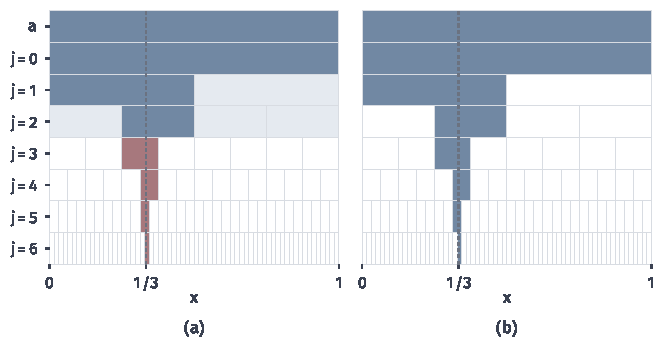
\includegraphics[width=112mm]{figures/04-spaces-measures-and-geometry/03-function-spaces/matplotlib/besov-haar-tiles/figure.pdf}
  \caption{$f=\mathbf 1_{[0,1/3)}$的Haar坐标，每个方格是一个基函数的位置和尺度，虚线标出跳跃点$x=1/3$。每层只有含跳跃点的方格系数非零。(a)固定尺度截断：浅蓝色是保留而系数为零的项，深蓝色是保留的非零项，红色是舍弃的非零项。(b)最佳$N$项：$N=8$项全部用在非零系数上。}
  \label{fig:besov-haar-tiles}
\end{BookInlineFigure}

两种做法的误差差别如表~\ref{tab:besov-fixed-vs-best}，图~\ref{fig:besov-error-decay}画出同样的数据。固定截断的误差按项数的$-1/2$次幂下降，最佳$N$项的误差按项数指数下降。

\begin{BookInlineTable}
  \centering
  \begin{tabular}{@{}cccccc@{}}
    \toprule
    项数 & $1$ & $2$ & $4$ & $8$ & $16$\\
    \midrule
    固定截断$E_J$（$M=2^J$） & $0.471$ & $0.333$ & $0.236$ & $0.167$ & $0.118$\\
    最佳$N$项$\sigma_N$ & $0.471$ & $0.333$ & $0.167$ & $0.042$ & $0.003$\\
    \bottomrule
  \end{tabular}
  \caption{$f=\mathbf 1_{[0,1/3)}$在Haar基下的两种误差。}
  \label{tab:besov-fixed-vs-best}
\end{BookInlineTable}

\begin{BookInlineFigure}
  \centering
  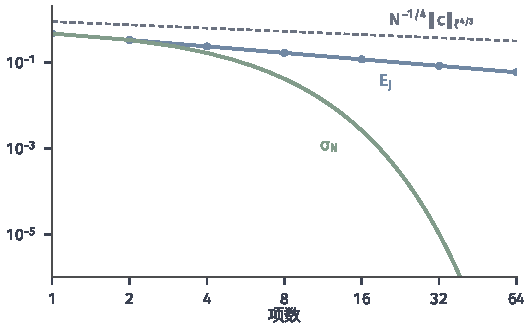
\includegraphics[width=90mm]{figures/04-spaces-measures-and-geometry/03-function-spaces/matplotlib/besov-error-decay/figure.pdf}
  \caption{同一函数的两种误差，双对数坐标。蓝色为固定截断$E_J$，圆点在$M=2^J$处；绿色为最佳$N$项误差$\sigma_N$；灰色虚线是定理~\ref{thm:besov-n-term-upper}在$s=1/4$时给出的上界。}
  \label{fig:besov-error-decay}
\end{BookInlineFigure}

换成更光滑的紧支撑小波，同样的现象仍然出现。设$\int\psi=0$。若$\psi_{j,k}$的支撑内部不含跳跃点，$f$在其上为常数，系数为零；含跳跃点的$k$每层只有有界个，并且
\[
 \lvert c_{j,k}\rvert\leq\lVert\psi_{j,k}\rVert_1=2^{-j/2}\lVert\psi\rVert_1 .
\]
所以每层只有有界个非零系数，大小按$2^{-j/2}$衰减，$\sigma_N$仍随$N$指数衰减。

固定截断则不然。阶跃函数不属于任何$s>1/2$的$B^s_{2,\infty}$，由定理~\ref{thm:besov-truncation-characterization}，$E_J(f)=O(2^{-Js})$对$s>1/2$不成立，用$M$个固定基函数的误差不能比$M^{-1/2}$快出一个幂次。

两种方式的差别在于保留哪些方向：固定截断按下标保留，自适应选择按大小保留。代价有两点。每个函数各自选择$N$个下标，要用有限个代表覆盖整个函数类时，还必须计入“选了哪些下标”这一信息。近似对$f$也不再是线性的：两个函数之和的最佳$N$项近似，一般不是各自近似之和。

\subsection{最佳\texorpdfstring{$N$}{N}项误差的上界}
\label{sec:besov-n-term-upper}

在$1/\tau=s+1/2$时，小波范数~\eqref{eq:besov-wavelet-norm}中$p=q=\tau$，权重$2^{j(s+1/2-1/\tau)}=1$完全抵消。组内和组间都用$\ell^\tau$，分组也就不再起作用：
\[
 \lVert f\rVert_{B^s_{\tau,\tau}}^{\mathrm w}=\lVert a\rVert_{\ell^\tau}+\Bigl(\sum_{j\geq j_0}\lVert c_j\rVert_{\ell^\tau}^\tau\Bigr)^{1/\tau}.
\]

记$c$为全部系数（包括有限个粗项）组成的序列。对非负数$A,B$有下面的比较：
\[
 (A^\tau+B^\tau)^{1/\tau}\leq A+B\leq2(A^\tau+B^\tau)^{1/\tau} .
\]
取$A=\lVert a\rVert_{\ell^\tau}$，$B$为细节部分的$\ell^\tau$范数，得到
\begin{equation}
 \lVert c\rVert_{\ell^\tau}\leq\lVert f\rVert^{\mathrm w}_{B^s_{\tau,\tau}}\leq2\lVert c\rVert_{\ell^\tau}.
 \label{eq:besov-ltau-coeff}
\end{equation}
所以$f\in B^s_{\tau,\tau}$恰好意味着全部系数$\tau$次可和，不再区分它们来自哪一层。

$\tau<2$时，$\ell^\tau$可和比平方可和更强。这与有限维中的现象相同：在单位$\ell^2$球面上，$\ell^\tau$范数小的向量大部分能量集中在少数分量上。表~\ref{tab:besov-concentrate-spread}中，$\tau=1$时集中的$c^{\mathrm A}$范数是$1$，分散的$c^{\mathrm B}$范数是$2^{3/2}$。

\begin{theorem}[最佳$N$项误差的上界]
\label{thm:besov-n-term-upper}
设$0<s<1/2$，$1/\tau=s+1/2$。则对每个$f\in L^2(\mathbb T)\cap B^s_{\tau,\tau}$和每个$N\geq1$，
\begin{equation}
 \sigma_N(f)_2\leq N^{-s}\lVert c\rVert_{\ell^\tau}\leq C_0N^{-s}\lVert f\rVert_{B^s_{\tau,\tau}} .
 \label{eq:besov-n-term-upper}
\end{equation}
\end{theorem}

\begin{proof}
重排序列的前$n$项都不小于$c_n^*$，所以$n(c_n^*)^\tau\leq\lVert c\rVert_{\ell^\tau}^\tau$，即
\[
 c_n^*\leq n^{-1/\tau}\lVert c\rVert_{\ell^\tau} .
\]

把式~\eqref{eq:besov-n-term-error}中每一项写成$(c_n^*)^2=(c_n^*)^{2-\tau}(c_n^*)^\tau$。$n>N$时$c_n^*\leq c_N^*$，于是
\[
 \sigma_N(f)_2^2\leq(c_N^*)^{2-\tau}\sum_{n>N}(c_n^*)^\tau\leq(c_N^*)^{2-\tau}\lVert c\rVert_{\ell^\tau}^\tau .
\]

代入$c_N^*$的上界，并用$(2-\tau)/\tau=2/\tau-1=2s$，得到
\[
 \sigma_N(f)_2^2\leq N^{-(2-\tau)/\tau}\lVert c\rVert_{\ell^\tau}^{2-\tau}\lVert c\rVert_{\ell^\tau}^\tau=N^{-2s}\lVert c\rVert_{\ell^\tau}^2 .
\]
第二个不等式由式~\eqref{eq:besov-ltau-coeff}与定理~\ref{thm:besov-wavelet-characterization}得到。
\end{proof}

用贯穿的例子核对。取$s=1/4$，则$\tau=4/3$。全部系数的$\ell^{4/3}$范数由几何级数给出：
\[
 \lVert c\rVert_{\ell^{4/3}}^{4/3}=3^{-4/3}\Bigl(1+\frac{1}{1-2^{-2/3}}\Bigr)\approx0.8557,\qquad\lVert c\rVert_{\ell^{4/3}}\approx0.890 .
\]
$N=8$时上界为$8^{-1/4}\times0.890\approx0.529$，实际误差$0.0417$远小于它。这个上界对整个球成立，它要照顾到最坏的函数，而这个例子的系数衰减得特别快。

图~\ref{fig:besov-parameter-map}把几个空间放到$(1/p,s)$平面上。竖线$p=2$上的点是上一节的$B^s_{2,q}$，球上的固定截断速率是$M^{-s}$。绿线上的点是$B^s_{\tau,\tau}$，球上的最佳$N$项速率是同样的$N^{-s}$。从竖线沿箭头移到绿线，速率不变，度量方式却换成了$\ell^\tau$：函数可以把大系数集中在少数位置，只要全部系数$\tau$次可和。

\begin{BookInlineFigure}
  \centering
  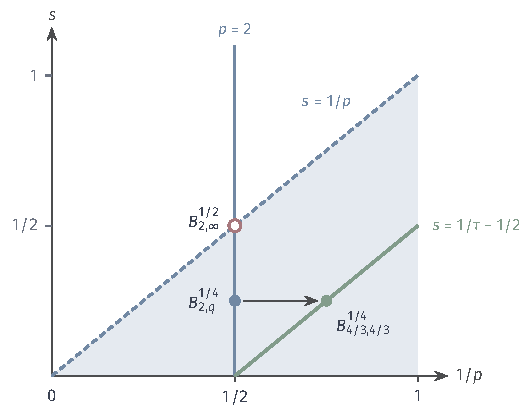
\includegraphics[width=90.1mm]{figures/04-spaces-measures-and-geometry/03-function-spaces/tikz/besov-parameter-map/figure.pdf}
  \caption{$(1/p,s)$平面上的Besov空间。蓝色竖线是$p=2$，绿线是$s=1/\tau-1/2$，箭头两端速率相同。虚线$s=1/p$是周期阶跃的临界线，其下方的浅蓝色区域内阶跃函数属于相应空间，红圈标出竖线上的临界点$B^{1/2}_{2,\infty}$。绿线整条位于浅蓝色区域内。}
  \label{fig:besov-parameter-map}
\end{BookInlineFigure}

图中还能读出阶跃函数为什么适合自适应逼近。在竖线上，阶跃函数的光滑阶数到$1/2$就停了。绿线却整条在临界线以下，因为$s=1/\tau-1/2<1/\tau$。在本节的范围$0<s<1/2$内，阶跃函数属于绿线上的每个空间。

\subsection{速率条件的逆向刻画}
\label{sec:besov-n-term-converse}

上界的反方向是：若误差满足$\sup_NN^s\sigma_N(f)_2<\infty$，函数是否属于$B^s_{\tau,\tau}$？答案是否定的，速率只对应一个更弱的条件。

\begin{theorem}[误差速率的刻画]
\label{thm:besov-n-term-rate}
设$s>0$，$1/\tau=s+1/2$，$f\in L^2(\mathbb T)$。则
\begin{equation}
 \sup_{N\geq1}N^s\sigma_N(f)_2<\infty\iff\sup_{n\geq1}n^{1/\tau}c_n^*<\infty .
 \label{eq:besov-n-term-rate}
\end{equation}
\end{theorem}

\begin{proof}
设$\sigma_N(f)_2\leq AN^{-s}$。第$N+1$到$2N$项共$N$项，都不小于$c_{2N}^*$，所以
\[
 N(c_{2N}^*)^2\leq\sum_{n=N+1}^{2N}(c_n^*)^2\leq\sigma_N(f)_2^2\leq A^2N^{-2s}.
\]
由此得到
\[
 c_{2N}^*\leq AN^{-s-1/2}=AN^{-1/\tau}.
\]
奇数下标用$c_{2N+1}^*\leq c_{2N}^*$，$n=1$用$c_1^*\leq\lVert f\rVert_2$，于是$\sup_nn^{1/\tau}c_n^*<\infty$。

反过来，设$c_n^*\leq Bn^{-1/\tau}$。代入式~\eqref{eq:besov-n-term-error}，用积分比较尾和，并用$2/\tau-1=2s>0$，得到
\[
 \sigma_N(f)_2^2\leq B^2\sum_{n>N}n^{-2/\tau}\leq B^2\int_N^\infty x^{-2/\tau}\,\mathrm dx=\frac{B^2N^{-2s}}{2s}.
\]
\end{proof}

条件$\sup_nn^{1/\tau}c_n^*<\infty$称为弱$\ell^\tau$条件，它比$\ell^\tau$可和弱。取$c_n^*=n^{-1/\tau}$，由$2/\tau=2s+1>1$，它平方可和，按任意次序放到基函数上就得到一个$L^2$函数$f$。它满足弱$\ell^\tau$条件，因而
\[
 \sigma_N(f)_2\leq(2s)^{-1/2}N^{-s}.
\]

可是$\sum_n(c_n^*)^\tau=\sum_nn^{-1}=\infty$，所以在$0<s<1/2$时$f\notin B^s_{\tau,\tau}$。单一的误差速率不能反推Besov成员资格，这与统一截断速率只对应$q=\infty$的情形相似。

\subsection{跨预算的误差汇总}
\label{sec:besov-approximation-spaces}

第~\ref{sec:besov-truncation-aggregation}小节看到，把截断误差跨尺度汇总可以恢复有限$q$的条件。对最佳$N$项误差也可以这样做：不只要求一个速率，而是把各个预算下的误差按$\ell^\tau$汇总。预算取二进值$N=2^m$。

\begin{definition}[逼近空间]
\label{def:besov-approximation-space}
设$s>0$，$1/\tau=s+1/2$。对$f\in L^2(\mathbb T)$，令
\begin{equation}
 \lVert f\rVert_{A^s_\tau}=\lVert f\rVert_2+\Bigl(\sum_{m\geq0}\bigl(2^{ms}\sigma_{2^m}(f)_2\bigr)^\tau\Bigr)^{1/\tau},
 \label{eq:besov-approximation-space}
\end{equation}
使其有限的函数组成的集合称为\term{逼近空间}（approximation space），记为$A^s_\tau$。
\end{definition}

$\sigma_N$随$N$单调不增，二进预算之间只差常数倍，所以$\sup_m2^{ms}\sigma_{2^m}(f)_2<\infty$等价于$\sup_NN^s\sigma_N(f)_2<\infty$。把上确界换成$\ell^\tau$和，正是把“统一速率”加强为“误差汇总”。

\begin{theorem}[逼近空间与Besov空间]
\label{thm:besov-approximation-equals-besov}
设$0<s<1/2$，$1/\tau=s+1/2$，小波满足定理~\ref{thm:besov-wavelet-characterization}的条件。则对$f\in L^2(\mathbb T)$，$f\in A^s_\tau$当且仅当$f\in B^s_{\tau,\tau}$，并且两个范数等价。
\end{theorem}

\begin{proof}
由式~\eqref{eq:besov-ltau-coeff}和定理~\ref{thm:besov-wavelet-characterization}，$\lVert f\rVert_{B^s_{\tau,\tau}}$与$\lVert c\rVert_{\ell^\tau}$等价，所以只需比较$\lVert f\rVert_{A^s_\tau}$与$\lVert c\rVert_{\ell^\tau}$。

先由系数控制误差汇总。由Parseval等式和$\tau<2$，$\lVert f\rVert_2$不超过$\lVert c\rVert_{\ell^\tau}$。把下标按二进块$2^l<n\leq2^{l+1}$分组，每块有$2^l$项，每项不超过$c_{2^l}^*$，所以
\[
 \sigma_{2^m}(f)_2^2\leq\sum_{l\geq m}2^l(c_{2^l}^*)^2 .
\]

记$\beta_l=2^{l/\tau}c_{2^l}^*$，则$2^l(c_{2^l}^*)^2=2^{-2ls}\beta_l^2$。乘以$2^{2ms}$并开方，得到
\[
 2^{ms}\sigma_{2^m}(f)_2\leq\Bigl(\sum_{l\geq m}2^{-2(l-m)s}\beta_l^2\Bigr)^{1/2}\leq\sum_{l\geq m}2^{-(l-m)s}\beta_l .
\]
由式~\eqref{eq:besov-convolution}，左端序列的$\ell^\tau$范数不超过$(1-2^{-s})^{-1}\lVert(\beta_l)\rVert_{\ell^\tau}$。

余下要用$\lVert c\rVert_{\ell^\tau}$控制$\lVert(\beta_l)\rVert_{\ell^\tau}$。$l\geq1$时，第$2^{l-1}+1$到$2^l$项共$2^{l-1}$项，都不小于$c_{2^l}^*$，所以
\[
 2^{l-1}(c_{2^l}^*)^\tau\leq\sum_{2^{l-1}<n\leq2^l}(c_n^*)^\tau .
\]
对$l$求和，并单独计入$\beta_0=c_1^*$，得到
\[
 \sum_{l\geq0}\beta_l^\tau\leq2\lVert c\rVert_{\ell^\tau}^\tau .
\]

再由误差汇总控制系数。下标$2^{m+1}\leq n<2^{m+2}$的块有$2^{m+1}$项，每项不超过$c_{2^{m+1}}^*$。由上一小节的论证，$2^m(c_{2^{m+1}}^*)^2\leq\sigma_{2^m}(f)_2^2$。所以
\[
 \begin{aligned}
 \sum_{n\geq2}(c_n^*)^\tau&\leq\sum_{m\geq0}2^{m+1}(c_{2^{m+1}}^*)^\tau\\
 &\leq2\sum_{m\geq0}2^{m(1-\tau/2)}\sigma_{2^m}(f)_2^\tau\\
 &=2\sum_{m\geq0}\bigl(2^{ms}\sigma_{2^m}(f)_2\bigr)^\tau ,
 \end{aligned}
\]
最后一步用了$\tau s=1-\tau/2$，它等价于$1/\tau=s+1/2$。

加上$c_1^*\leq\lVert f\rVert_2$，得到
\[
 \lVert c\rVert_{\ell^\tau}^\tau\leq\lVert f\rVert_2^\tau+2\lVert f\rVert_{A^s_\tau}^\tau .
\]
\end{proof}

这个定理说明，比统一速率更强的误差汇总恰好恢复了系数的强可和性。它依赖本节固定的条件：同一正交小波基，$L^2$误差，$1/\tau=s+1/2$，以及满足小波刻画条件的小波。换成冗余字典、其他误差范数或不匹配的指数，都需要另行分析。

\section{Besov球的覆盖数}
\label{sec:besov-covering}

前两节回答的是“给一个函数，用多少项能达到给定误差”。另一类问题是：为整类函数预先准备有限个代表，使类中每个函数都离某个代表足够近，至少需要多少个代表？第~\ref{chap:sobolev-spaces}章的紧嵌入只说明Sobolev球的覆盖数有限，没有给出增长阶。本节回到第~\ref{sec:besov-scale-truncation}节的$B^s_{2,q}$有界类，在$L^2$距离下算出覆盖数随精度的增长：固定尺度截断控制尾部，逐尺度覆盖保留的系数给出上界，再用只在单一尺度上变化的子类给出同阶的下界。

\subsection{函数类、距离与精度}
\label{sec:besov-cover-setting}

固定单位周期、$s>0$、$1\leq q\leq\infty$与$R>0$，令
\[
\mathcal F_R=\{f\in L^2(\mathbb T):\lVert f\rVert_{B^s_{2,q}}\leq R\}.
\]
沿用第~\ref{chap:metric-spaces}章的覆盖数：记$N(\varepsilon,\mathcal F_R)$为覆盖$\mathcal F_R$所需的半径为$\varepsilon$的$L^2$闭球的最少个数，球心可以取在整个$L^2(\mathbb T)$中。若要求球心属于$\mathcal F_R$，由那里的比较$N_X(\varepsilon,A)\leq N_A(\varepsilon,A)\leq N_X(\varepsilon/2,A)$，只需把半径调整一个固定的因子，下面的增长阶不变。

我们关心$\varepsilon\to0$时$\log N(\varepsilon,\mathcal F_R)$怎样增长，即度量熵。$\mathcal F_R$在$L^2$中全有界：统一截断界说明它离有限维子空间$V_J$一致地近，而它在$V_J$上的投影是有界集。下面把这个定性论证做成定量计数。

\subsection{逐尺度精度分配}
\label{sec:besov-precision-allocation}

由第~\ref{sec:besov-uniform-truncation}小节，类中每个函数满足$E_J(f)\leq C_sR2^{-Js}$，并且由式\eqref{eq:besov-wavelet-norm-l2}，每层系数满足$\lVert a\rVert_{\ell^2}\leq C_0R$，$\lVert c_j\rVert_{\ell^2}\leq C_0R2^{-js}$。覆盖的构造分两部分：尾部直接舍去，保留的系数逐层覆盖。

\emph{尾部。}设$0<\varepsilon<2C_sR\,2^{-(j_0+1)s}$，取$J$为使$C_sR2^{-Js}\leq\varepsilon/2$的最小整数。这一假设保证$J>j_0+1$，并且由最小性$C_sR2^{-(J-1)s}>\varepsilon/2$。于是每个函数的尾部误差$E_J(f)\leq\varepsilon/2$，并且
\begin{equation}
\frac{R}{\varepsilon}\leq\frac{2^{Js}}{2C_s},\qquad2^J<2\Bigl(\frac{2C_sR}{\varepsilon}\Bigr)^{1/s}.
\label{eq:besov-cover-scale}
\end{equation}

\emph{保留的系数。}把粗项$a$并入起始一层，组成维数为$2^{j_0}+2^{j_0}=2^{j_0+1}$的块$(a,c_{j_0})$，半径至多$\sqrt2C_0R$；其余每个$j_0<j<J$的块$c_j$维数为$2^j$，半径至多$C_0R2^{-js}$。对第$j$块分配覆盖精度
\[
\delta_j=\frac\varepsilon2\,2^{-(J-j)/2},\qquad j_0\leq j<J .
\]
越粗的层分到越大的精度，因为它们半径大而维数小；越接近截断尺度的层精度越细。总和满足
\[
\sum_{j_0\leq j<J}\delta_j^2=\frac{\varepsilon^2}{4}\sum_{j_0\leq j<J}2^{-(J-j)}<\frac{\varepsilon^2}{4}\sum_{m\geq1}2^{-m}=\frac{\varepsilon^2}4 .
\]

\emph{合并。}对每块取一个$\delta_j$覆盖，从每块的覆盖中各选一个中心，组成$V_J$中的一个函数$g$。给定$f\in\mathcal F_R$，在每块中选取与$f$的该块系数相距不超过$\delta_j$的中心。由正交性，误差的平方等于各块误差平方与尾部误差平方之和：
\[
\lVert f-g\rVert_2^2\leq\sum_{j_0\leq j<J}\delta_j^2+E_J(f)^2<\frac{\varepsilon^2}4+\frac{\varepsilon^2}4<\varepsilon^2 .
\]
所以这些组合中心构成$\mathcal F_R$的$\varepsilon$覆盖，个数是各块覆盖个数的乘积。

\subsection{对数覆盖数的上界}
\label{sec:besov-entropy-upper}

现在计数。每块通过正交坐标等距地对应于欧氏空间中的球。由第~\ref{chap:metric-spaces}章，$n$维实赋范空间中半径为$\rho$的闭球可以用不超过$(1+2\rho/\delta)^n$个半径为$\delta$的闭球覆盖。

\begin{theorem}[对数覆盖数的上界]
\label{thm:besov-entropy-upper}
设$s>0$，$1\leq q\leq\infty$。存在只依赖$s,q$与所选小波的常数$c,C>0$，使对$0<\varepsilon\leq cR$，
\[
\log N(\varepsilon,\mathcal F_R)\leq C\Bigl(\frac R\varepsilon\Bigr)^{1/s}.
\]
\end{theorem}

\begin{proof}
取$c=C_s2^{-(j_0+1)s}$，则$\varepsilon\leq cR$保证上一小节的假设成立。记$\rho_j$为第$j$块的半径。对$j_0<j<J$，由式\eqref{eq:besov-cover-scale}与$C_0\leq C_s$，
\[
\frac{2\rho_j}{\delta_j}\leq\frac{4C_0R\,2^{-js}2^{(J-j)/2}}{\varepsilon}\leq\frac{2C_0}{C_s}2^{(J-j)s}2^{(J-j)/2}\leq2\cdot2^{(J-j)(s+1/2)},
\]
所以$\log(1+2\rho_j/\delta_j)\leq\log3+(J-j)(s+1/2)\log2\leq C_1(1+J-j)$。起始块的半径多一个因子$\sqrt2\,2^{j_0s}$，只改变常数。按块相乘再取对数，
\[
\log N(\varepsilon,\mathcal F_R)\leq\sum_{j_0\leq j<J}2^{j+1}C_1(1+J-j)\leq2C_1\,2^J\sum_{m\geq1}2^{-m}(1+m)=6C_1\,2^J ,
\]
这里令$m=J-j$，并用了$\sum_{m\geq1}2^{-m}=1$与$\sum_{m\geq1}m2^{-m}=2$。再由式\eqref{eq:besov-cover-scale}，$2^J<2(2C_sR/\varepsilon)^{1/s}$，即得结论。
\end{proof}

估计的对象是对数覆盖数，不是覆盖数本身：覆盖数按$\exp(C(R/\varepsilon)^{1/s})$增长。计数的主要部分来自接近截断尺度的几层，那里维数最大；每层贡献“维数乘以$1+J-j$”，几何权重使总和与最细保留层的维数$2^J$同阶。常数依赖固定的$s,q$与小波，适用范围是$0<\varepsilon\leq cR$；$\varepsilon$与$R$同阶或更大时，少数几个代表就够了。

\subsection{覆盖数的下界}
\label{sec:besov-entropy-lower}

上界是否太粗？我们用一个只在单一尺度上变化的子类核对。

\begin{theorem}[对数覆盖数的下界]
\label{thm:besov-entropy-lower}
在定理~\ref{thm:besov-entropy-upper}的条件下，存在常数$c',c''>0$，使对$0<\varepsilon\leq c''R$，
\[
\log N(\varepsilon,\mathcal F_R)\geq c'\Bigl(\frac R\varepsilon\Bigr)^{1/s}.
\]
\end{theorem}

\begin{proof}
令$\alpha=1/C_0$。对$j\geq j_0$，考虑只允许第$j$层系数变化、其余系数为零的函数$f=\sum_kx_k\psi_{j,k}$，$\lVert x\rVert_{\ell^2}\leq\alpha R2^{-js}$。它的系数范数为$2^{js}\lVert x\rVert_{\ell^2}\leq\alpha R$，所以$\lVert f\rVert_{B^s_{2,q}}\leq C_0\alpha R=R$，这些函数组成$\mathcal F_R$的子集$\mathcal G_j$。$\mathcal G_j$等距于$2^j$维欧氏空间中半径$\rho=\alpha R2^{-js}$的闭球。

覆盖$\mathcal F_R$的球也覆盖$\mathcal G_j$。到第$j$层子空间的正交投影不增大与该子空间中点的距离，所以可以把球心都投影到这个子空间中。$N$个半径$\varepsilon$的球覆盖半径$\rho$的球，比较体积得$N\varepsilon^{2^j}\geq\rho^{2^j}$，即$\log N\geq2^j\log(\rho/\varepsilon)$。

选择尺度：数列$\alpha R2^{-js}$（$j\geq j_0$）每步缩小因子$2^s$，若$\varepsilon\leq\alpha R2^{-j_0s}/4$，则恰有一个$j$满足$4\varepsilon\leq\alpha R2^{-js}<2^{s+2}\varepsilon$。对这个$j$，$\rho/\varepsilon\geq4$，所以$\log N\geq2^j\log4$；又$2^{js}>\alpha R/(2^{s+2}\varepsilon)$，即$2^j>(\alpha/2^{s+2})^{1/s}(R/\varepsilon)^{1/s}$。合并即得结论，$c'=\log4\cdot(\alpha/2^{s+2})^{1/s}$。
\end{proof}

上下界合起来，$\log N(\varepsilon,\mathcal F_R)$与$(R/\varepsilon)^{1/s}$同阶，增长阶由光滑阶数$s$决定，与汇总指数$q$无关：$q$改变球的大小，但单尺度子类与逐尺度上界只用到每层的统一界，两端的量级相同。这个结论依赖本节固定的设定，即单位周期、$p=2$的Besov球与$L^2$距离；其他积分指数、误差范数或区域需要另行分析，例如目标范数与$p$不同时，单尺度子类不再是欧氏球。与Sobolev紧嵌入只给出“有限”相比，这里的小波坐标把函数类分解为一串维数与半径都已知的有限维球，计数因而可以完成。

\section{与Sobolev空间的联系}
\label{sec:besov-sobolev}

Besov空间是为补充Sobolev条件而引入的，自然要问二者在重合处是否一致。本节只对照第~\ref{chap:sobolev-spaces}章已经定义的一阶平方可积弱导数：在单位周期设定下，$B^1_{2,2}$恰好由端点值相同的$H^1(0,1)$函数组成，范数等价。随后说明端点条件与二阶差分各自为何必要，再用其他参数说明Besov空间在Sobolev空间之外增加了什么。

\paragraph{定理与证明}
记$H^1_{\mathrm{per}}=\{f\in H^1(0,1):\tilde f(0)=\tilde f(1)\}$，其中$\tilde f$是$f$的绝对连续代表，这类函数按周期$1$延拓后在接缝处连续。

\begin{theorem}[$B^1_{2,2}$与周期$H^1$]
\label{thm:besov-b122-h1}
在单位周期上，$B^1_{2,2}(\mathbb T)=H^1_{\mathrm{per}}$，并且存在常数$C$，使$C^{-1}\lVert f\rVert_{H^1(0,1)}\leq\lVert f\rVert_{B^1_{2,2}}\leq C\lVert f\rVert_{H^1(0,1)}$。
\end{theorem}

证明借助周期Fourier系数$\widehat f(k)=\int_0^1f(x)e^{-2\pi\mathrm ikx}\,\mathrm dx$，分两步：先说明$H^1_{\mathrm{per}}$恰好由$\sum_kk^2|\widehat f(k)|^2<\infty$的函数组成，再说明$B^1_{2,2}$的半范数平方与这个和等价。

\emph{第一步：Fourier系数刻画$H^1_{\mathrm{per}}$。}设$f\in H^1_{\mathrm{per}}$。对绝对连续代表分部积分，
\begin{equation*}
\begin{aligned}
\widehat{f'}(k)&=\Bigl[\tilde f(x)e^{-2\pi\mathrm ikx}\Bigr]_0^1+2\pi\mathrm ik\int_0^1\tilde f(x)e^{-2\pi\mathrm ikx}\,\mathrm dx\\
&=\bigl(\tilde f(1)-\tilde f(0)\bigr)+2\pi\mathrm ik\,\widehat f(k)=2\pi\mathrm ik\,\widehat f(k),
\end{aligned}
\end{equation*}
端点条件正好消去边界项。由Parseval等式，$\lVert f'\rVert_2^2=4\pi^2\sum_kk^2|\widehat f(k)|^2<\infty$。反过来，设$\sum_kk^2|\widehat f(k)|^2<\infty$，则$g=\sum_k2\pi\mathrm ik\widehat f(k)e^{2\pi\mathrm ikx}\in L^2$，且$\widehat g(0)=0$。令$F(x)=c+\int_0^xg$，常数$c$使$\int_0^1F=\widehat f(0)$。$F$绝对连续，$F(1)-F(0)=\widehat g(0)=0$；对$k\neq0$分部积分得$\widehat F(k)=\widehat g(k)/(2\pi\mathrm ik)=\widehat f(k)$。Fourier系数全部相同，由完备性$F=f$几乎处处，所以$f\in H^1_{\mathrm{per}}$。

\emph{第二步：半范数与系数和等价。}$s=1$时须取$r\geq2$，这里取$r=2$。由式\eqref{eq:besov-difference-fourier}，$\lVert\Delta_h^2f\rVert_2^2=\sum_k(2|\sin(\pi kh)|)^4|\widehat f(k)|^2$。下界：$\omega_2(f,t)_2\geq\lVert\Delta_t^2f\rVert_2$，交换求和与积分，
\[
|f|_{B^1_{2,2}}^2\geq\sum_k|\widehat f(k)|^2\int_0^1t^{-3}\,16\sin^4(\pi kt)\,\mathrm dt .
\]
对$k\neq0$换元$u=|k|t$，内层积分等于$k^2\int_0^{|k|}16u^{-3}\sin^4(\pi u)\,\mathrm du\geq c_1k^2$，其中$c_1=16\int_0^1u^{-3}\sin^4(\pi u)\,\mathrm du$为正的有限数（被积函数在$u\to0$时约为$\pi^4u$）。上界：$(2|\sin(\pi kh)|)^4\leq\min\bigl(16,(2\pi|k||h|)^4\bigr)$，右端随$|h|$不减，所以$\omega_2(f,t)_2^2\leq\sum_k\min(16,(2\pi|k|t)^4)|\widehat f(k)|^2$；同样换元，$\int_0^1t^{-3}\min(16,(2\pi|k|t)^4)\,\mathrm dt\leq C_1k^2$，$C_1=\int_0^\infty u^{-3}\min(16,(2\pi u)^4)\,\mathrm du<\infty$。于是
\[
c_1\sum_kk^2|\widehat f(k)|^2\leq|f|_{B^1_{2,2}}^2\leq C_1\sum_kk^2|\widehat f(k)|^2 .
\]
两步合并，$f\in B^1_{2,2}$当且仅当$f\in H^1_{\mathrm{per}}$，且$|f|_{B^1_{2,2}}$与$\lVert f'\rVert_2$等价；再加上$\lVert f\rVert_2$，两个范数等价。

\paragraph{端点条件的作用}
不能把全部$H^1(0,1)$当作周期空间。$f(x)=x$属于$H^1(0,1)$，但$\tilde f(0)=0\neq1=\tilde f(1)$，按周期延拓后在每个整数点跳跃。直接计算，$k\neq0$时$\widehat f(k)=-1/(2\pi\mathrm ik)$，于是$k^2|\widehat f(k)|^2=1/(4\pi^2)$不可和，$f\notin B^1_{2,2}$。它的系数与周期阶跃同样按$1/|k|$衰减，周期延拓后的光滑阶数只有$1/2$。第一步的分部积分清楚地显示了原因：边界项$\tilde f(1)-\tilde f(0)$不为零时，$\widehat{f'}(k)$与$2\pi\mathrm ik\widehat f(k)$相差一个常数，这个常数正是接缝处的跳跃。

\paragraph{二阶差分的必要性}
$s=1$时差分阶数必须取$r\geq2$。若用一阶差分，由第~\ref{sec:besov-modulus}小节的饱和现象，任何非常数的$f$都有某个$\widehat f(k)\neq0$，$k\neq0$；当$|k|t\leq1/2$时，$\omega_1(f,t)_2\geq2|\sin(\pi kt)||\widehat f(k)|\geq4|k|t|\widehat f(k)|$，所以$t^{-1}\omega_1(f,t)_2$在小$t$处有正的下界，$\int_0(t^{-1}\omega_1)^2\,\mathrm dt/t$发散。用一阶差分写出的“$B^1_{2,2}$”只含常数。小波刻画也有同样的要求：所用小波须有超过一阶的正则性与消失矩，Haar小波不能用于$s=1$。

\paragraph{其他参数}
同样的Fourier计算适用于其他光滑阶数。$0<s<1$时取$r=1$，$\int_0^1t^{-1-2s}4\sin^2(\pi kt)\,\mathrm dt$与$|k|^{2s}$同阶，所以$B^s_{2,2}$由$\sum_k(1+k^2)^s|\widehat f(k)|^2<\infty$刻画，它是分数阶的平方可积光滑性，整数阶的$H^1_{\mathrm{per}}$是其中$s=1$的情形。可以证明，对正整数$s$，$B^s_{2,2}$与$s$阶的周期$H^s$一致，这里不给出证明。

$p\neq2$时情况不同。对$1<p<\infty$，可以证明周期的$W^{1,p}$介于$B^1_{p,\min(p,2)}$与$B^1_{p,\max(p,2)}$之间，一般不等于任何一个$B^1_{p,q}$；整数阶Sobolev空间与Besov空间只在$p=2$时简单重合。这一结论这里不给出证明。

Besov空间在Sobolev空间之外增加的，正是本章开头要求的两项描述。光滑阶数$s$可以取分数，于是没有弱导数的周期阶跃也有确切位置：它属于$B^{1/2}_{2,\infty}$，并属于每个$s<1/2$的$B^s_{2,q}$。汇总指数$q$可以选择，于是只在统一速率上相同、跨尺度分布不同的函数，例如第~\ref{sec:besov-distribution-aggregation}小节的两种权重，或例~\ref{ex:besov-one-coefficient-per-scale}，可以被区分开。积分指数$p$则与$s$配合，决定像$B^s_{\tau,\tau}$那样允许稀疏大系数的空间，这对应于最佳$N$项逼近。

\section{本章小结}
\label{sec:besov-summary}

本章开头指出了一阶Sobolev条件的两处空白：它排除了阶跃函数，却读不出阶跃函数平移差的规律；它也没有规定不同尺度上的变化怎样汇总。平移差回答了第一点：周期阶跃在$L^2$中满足$\lVert\Delta_hf\rVert_2=(2|h|)^{1/2}$，光滑性可以是步长的分数次幂。同一尺度上，积分指数$p$决定位置不同的变化怎样度量，集中在小集合上的变化在大$p$下显得更剧烈；跨尺度上，统一上界看不出变化在多少个尺度上持续出现，需要单独的汇总方式。高阶差分抵消局部低阶多项式，连续模取步长不超过给定尺度的最坏情形；饱和现象说明$r$阶连续模至多表达$r$阶规律，所以刻画$s$阶光滑性须用$r>s$阶差分。

Besov范数把$t^{-s}\omega_r(f,t)_p$按$\mathrm dt/t$的$L^q$方式汇总，再加上$\lVert f\rVert_p$。$s$规定期望的变化阶数，$p$汇总同层位置，$q$汇总不同尺度；周期阶跃在$s<1/2$时属于每个$B^s_{2,q}$，在$s=1/2$时只属于$B^{1/2}_{2,\infty}$，清楚地分开了$s$与$q$的作用。完备性先在$L^p$中取极限，再借差分的连续性与Fatou引理把差分估计传到极限。小波刻画把同样的要求改写为系数条件：第$j$层的加权块大小$2^{j(s+1/2-1/p)}\lVert c_j\rVert_{\ell^p}$按$\ell^q$汇总，再加上粗项。等价性要求小波的正则性与消失矩都高于$s$，Haar小波只适用于较小的$s$。

在小波坐标中，三种逼近任务分别由不同条件控制。固定尺度截断为整类函数预先选定$2^J$维子空间，$B^s_{2,q}$球上的统一误差为$C_sRM^{-s}$，与$q$无关；反过来，截断误差序列$(2^{Js}E_J(f))_J$的$\ell^q$汇总恰好刻画$B^s_{2,q}$，单一的统一速率只对应$q=\infty$。最佳$N$项逼近让每个函数自选下标；在$1/\tau=s+1/2$时，$B^s_{\tau,\tau}$就是系数的$\ell^\tau$可和性，它给出$\sigma_N(f)_2\leq CN^{-s}$。误差速率本身只等价于弱$\ell^\tau$条件，不能反推Besov成员资格；把各个预算的误差按$\ell^\tau$汇总得到的逼近空间$A^s_\tau$，才与$B^s_{\tau,\tau}$一致。

整类函数的有限覆盖是第三种任务。对$B^s_{2,q}$球，先由统一截断界舍去尾部，再对保留的各层按几何方式分配精度，用有限维球的覆盖界逐层计数，得到$\log N(\varepsilon,\mathcal F_R)\leq C(R/\varepsilon)^{1/s}$；只在单一尺度上变化的子类是一个欧氏球，体积比较给出同阶的下界。与Sobolev紧嵌入只给出“有限”不同，这里得到了增长阶，它由$s$决定而与$q$无关。误差速率、误差汇总与对数覆盖数回答不同的问题，各自需要的参数条件不能相互替代。

最后，在单位周期上$B^1_{2,2}$与端点值相同的$H^1(0,1)$函数一致，范数等价；端点条件消去分部积分的边界项，二阶差分避开一阶连续模的饱和。$p\neq2$时整数阶Sobolev空间一般不与Besov空间重合。Besov尺度在Sobolev空间之外增加的，是分数的变化阶数、可选的尺度汇总，以及与稀疏逼近相匹配的积分指数。从离散观测出发、具有连续点值读取的函数空间，是第~\ref{chap:rkhs}章的对象。

